\documentclass[xcolor=x11names]{beamer}

\usetheme{metropolis}           % Use metropolis them
\usecolortheme{metropolis}

%Defining the theme
% \usetheme{Madrid}
% \useoutertheme[subsection=true,shadow]{miniframes}
%  \useinnertheme{circles}
%  \usepackage{etoolbox}
%  \usepackage{calc}

\definecolor{TaridesDarkBlue}{RGB}{10, 63, 92}
\definecolor{TaridesMidDarkBlue}{RGB}{1, 91, 140} %015B8C
%\definecolor{TaridesMidDarkBlue}{RGB}{2, 113, 168} %0271A8
\definecolor{TaridesMidBlue}{RGB}{3, 150, 216}   % 0396D8
\definecolor{TaridesBrightBlue}{RGB}{55, 180, 236} % 37B4EC
\definecolor{TaridesLightBlue}{RGB}{144, 216, 252} % 90D8FC

% \setbeamercolor{palette primary}{bg=TaridesDarkBlue,fg=white}
% \setbeamercolor{palette secondary}{bg=TaridesLightBlue,fg=white}
% \setbeamercolor{palette tertiary}{bg=TaridesMidBlue,fg=white}
% \setbeamercolor{palette quaternary}{bg=TaridesBrightBlue,fg=white}
%\setbeamercolor{structure}{fg=TaridesDarkBlue} % itemize, enumerate, etc
%\setbeamercolor{section in toc}{fg=TaridesDarkBlue} % TOC sections
%\setbeamercolor*{frametitle}{fg=black,bg=DeepSkyBlue4}
%\setbeamercolor*{lower separation line head}{bg=black}


% Various packages
\usepackage[utf8]{inputenc}
\usepackage[french]{babel}
\usepackage[T1]{fontenc}
\usepackage{lmodern}
\usepackage{enumitem}
\usepackage{amsmath,amssymb,amsfonts}
\usepackage{xcolor}
\usepackage{listings,lstautogobble}
\usepackage{courier}
\lstset{language=caml,autogobble=true,
        commentstyle=\color{TaridesBrightBlue},
        basicstyle=\footnotesize\ttfamily,
        breaklines=true, 
        morekeywords={val},
        morekeywords=[2]{int, string, file_perm, unit, dir_handle, file_descr, open_flag, bytes, bool, option, list},
        keywordstyle=[2]{\color{TaridesMidDarkBlue}}
        }
        
\usepackage{graphicx}
\usepackage{pifont}
\usepackage{hyperref}

\AtBeginSubsection[]
{
 \begin{frame}
  \vfill
  \centering
  %\begin{beamercolorbox}[sep=8pt,center,shadow=true,rounded=true]{title}
    \usebeamerfont{title}\insertsubsectionhead\par%
  %\end{beamercolorbox}
  \vfill
  \end{frame}}

\setbeamertemplate{blocks}[rounded][shadow=true]
\setbeamertemplate{itemize subitem}[bullet]

\newcommand{\added}[1]{\textcolor{gray!60!cyan}{#1}}
\newcommand{\subtt}[1]{\textcolor{gray!30!cyan}{#1}}

\newcommand\wip{\textcolor{red}{Work in progress }}
\newcommand\todo[1]{\textcolor{red}{\textit{\small{#1}}}}

\title[Programmation système en OCaml]{Programmation système en OCaml : introduction et cas d'usage.}
\author[Carine et Lucas]{Carine Morel et Lucas Pluvinage}
\institute{Tarides}

\begin{document}
\maketitle

\begin{frame}{Tarides}

    \begin{itemize}[label=$-$]
        \item on fait des logiciels et du service en OCaml
        \item 70 employés (France, UK, USA, Inde etc..)
        \item tout en open source !  
    \end{itemize}
    
\begin{columns} 
    \column{0.3\linewidth} 
    \centering
    
\includegraphics[width=\textwidth]{slides/images/logo-TARIDES.png}

    \column{0.5\linewidth}
    \centering
    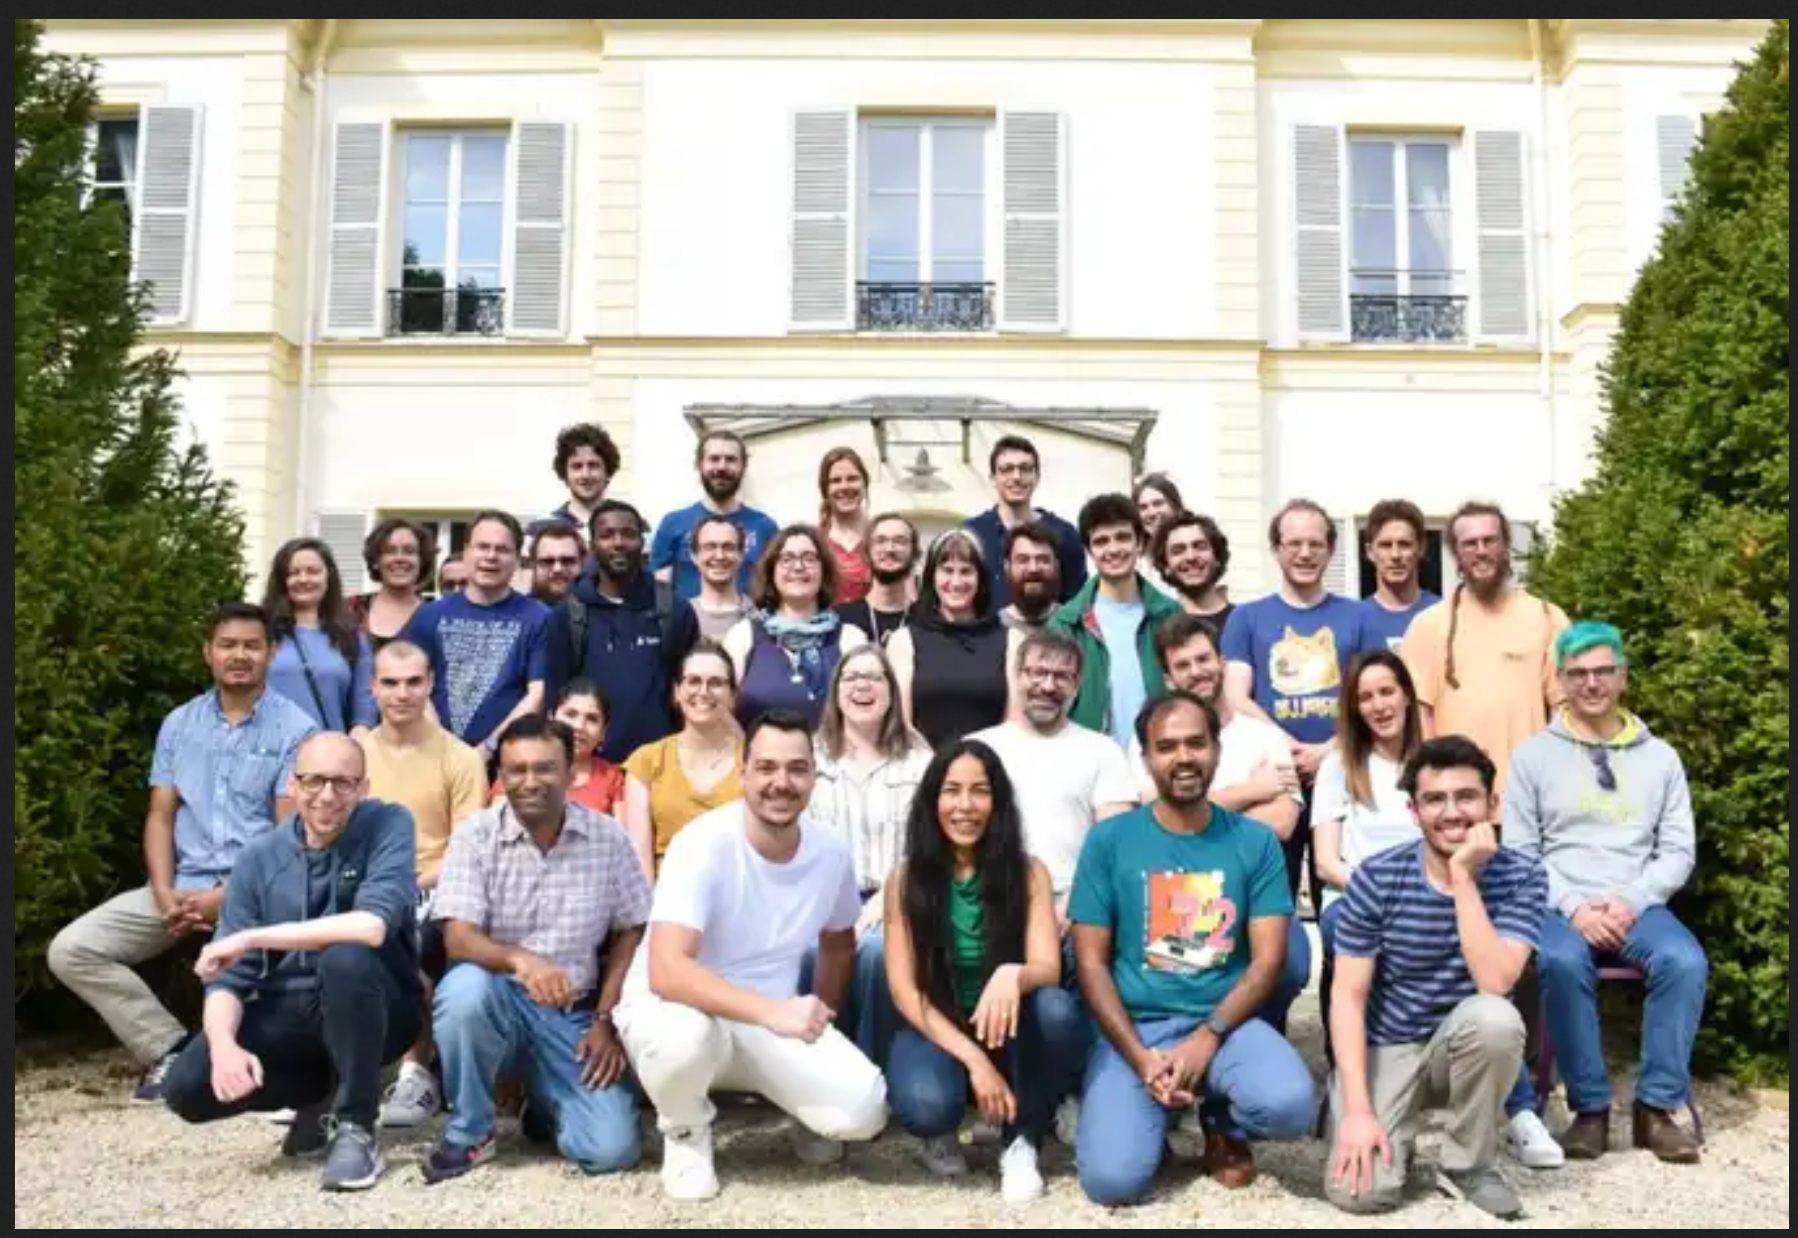
\includegraphics[width=\textwidth]{slides/images/tarides_team.png}
\end{columns}

\end{frame}

\begin{frame}{Plan}
   \subtt{Programmation système en OCaml} 
   
   \ding{217} autour de l'écriture d'un "mini" shell :
    \begin{itemize}[label=\ding{114}]
        \item le module Unix
        \item les processus Unix  
        \item et plus
    \end{itemize}   
    
    \ding{217} les algos d'exclusion mutuelle en OCaml

    \subtt{OCaml dans la vraie vie} 
     \begin{itemize}[label=$-$]
        \item Mirage : \textbf{un} système en OCaml
        \item QCheck : un vérificateur de propriétés automatiques
        \item OCaml 5.0
        \item Écosystème OCaml
    \end{itemize}   
\end{frame}

\section{Programmation système en OCaml}

\begin{frame}{Introduction : mini-shell}

    \subtt{Objectif :} programmer un shell en utilisant le module \texttt{Unix} 
    
    \todo{Screenshot d'un shell}
    
    Les fonctionnalités et commandes que l'on va implémenter :
    \begin{itemize}[label=\small\ding{114}]
        \item<1-> Manipulation des fichiers : \texttt{ls}, \texttt{mkdir}, \texttt{ln}, \texttt{cat}
        \item<1-> Modification du répertoire courant : \texttt{cd}
        \item<1-> Processus et environnement % entrée/sortie standard, fork
        \item<1-> Re-directions de flux :  $>$, $<$
        \item<1-> Tube : $|$

        %\item<2-> Pour aller plus loin : 
        %    \begin{itemize}[label=$-$]
        %        \item un peu de \textit{réseau}
        %        \item les sur-couches au module \texttt{Unix} : \textit{Lwt / Bos}
        %    \end{itemize}
    \end{itemize}
\end{frame}

\begin{frame}{Programmation système en OCaml}

    \begin{itemize}[label=\small\ding{114}]
        \item Des modules bas niveau (cf \url{ocaml.org/api})
            \begin{itemize}[label=\small\ding{118}]
                \item \texttt{Sys} : fonctions communes à Unix et aux autres OS sous lesquels tourne OCaml,
                \item \texttt{Unix} : fonctions spécifiques à Unix.
            \end{itemize}
        \item Des sur-couches sur le module \texttt{Unix} :
            \begin{itemize}[label=\small\ding{118}]
                \item certaines fonctions de la \texttt{Sdtlib}, 
                \item \texttt{Lwt.Unix}, 
                \item \texttt{Bos} etc..
            \end{itemize}
        \item Des modules utilitaires comme \texttt{Filename}
    \end{itemize}

\end{frame}

\begin{frame}{Module \texttt{Sys}}
    \begin{itemize}[label=\small\ding{114}]
        \item \wip
    \end{itemize}
\end{frame}

\subsection{Manipulation de fichiers et répertoires}
\begin{frame}[fragile]{Manipulation de fichiers et répertoire : interface du mini-shell}
    \begin{itemize}[leftmargin=-12pt]
    \item<1->Première version de l'AST des commandes :
        \todo{reorganiser dans l'ordre le plus pertinent en fonction de la suite}
        \begin{lstlisting}[breaklines=false]
            type command =
              | Cat of string list           (* cat files *)  
              | Ln of string * string * bool (* ln source dest [-s] *)
              | Mv of string * string        (* mv source dest *)
              | Rm of string * bool          (* rm filename [-r] *)  
              | Mkdir of string * int option (* mkdir dir [-m int] *)
              | Ls of string option          (* ls [filename] *)  
        \end{lstlisting}
        
    \item<2-> Parser, et interpréteur de commandes :
         \begin{lstlisting}
            val parse : string -> command
            val exec_command : command -> unit 
        \end{lstlisting}
    \end{itemize}
\end{frame}  

\begin{frame}[fragile]{Parseur et interpréteur}

    \begin{itemize}[label=\small\ding{114}]
    \item Parseur : plusieurs solutions (\texttt{Args}, \texttt{Angstrom} etc..)
    \item Interpréteur : 
      \begin{lstlisting}
            let exec_command cmd = 
                match cmd with
                | Cat filename              -> failwith "todo"
                | Ln (source, dest, symb)   -> failwith "todo"
                | Mv (source, dest)         -> failwith "todo"
                | Mkdir (dirname, perm_opt) -> failwith "todo"
                | Rm (filename, recursive)  -> failwith "todo"
                | Ls name_opt               -> failwith "todo"
        \end{lstlisting}
    \end{itemize}
\end{frame} 


\begin{frame}[fragile]{Lecture et écriture de fichier (\texttt{cat})}
    \texttt{cat f1 f2 f3}~... : concatène le contenu des fichiers en entrée et les écrit dans la sortie standard.
    
    \subtt{Exemple}
    
    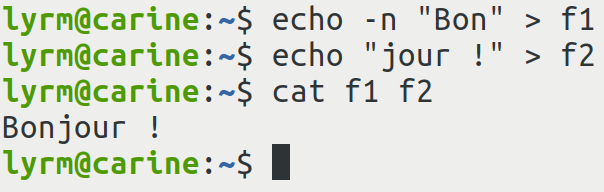
\includegraphics[width=0.5\textwidth]{slides/images/shell_cat.png}
    
    \pause\subtt{Pseudo-code}

    Pour chaque fichier en entrée : 
    \begin{itemize}[label=\small\ding{114}]
        \item ouvrir le fichier
        \item le lire et l'écrire sur la sortie standard
        \item fermer le fichier
    \end{itemize}
\end{frame}

\begin{frame}[fragile]{Lecture et écriture de fichier (\texttt{cat})}
    \begin{lstlisting}
        type file_descr         (* descripteurs de fichiers *)
        val stdin : file_descr  (* entree standard *)
        val stdout : file_descr (* sortie standard *)
        val stderr : file_descr (* sortie d'erreur standard *)
        
        type open_flag = (* modes d'ouverture *)
            | O_RDONLY  | O_WRONLY | O_RDWR
            | O_CREAT   | O_TRUNC 
         (* |.. et tous les autres  *)
        type file_perm = int (* droits (Ex : 0o777) *)
        
        val openfile : 
            string -> open_flag list -> file_perm -> file_descr
        val close : file_descr -> unit
        val read : file_descr -> bytes -> int -> int -> int
        val single_write : file_descr -> bytes -> int -> int -> int
    \end{lstlisting}
\end{frame}

\begin{frame}[fragile]{OCaml vs C : \texttt{write}}
    \begin{lstlisting}
        val single_write : file_descr -> bytes -> int -> int -> int    
    \end{lstlisting}
    
    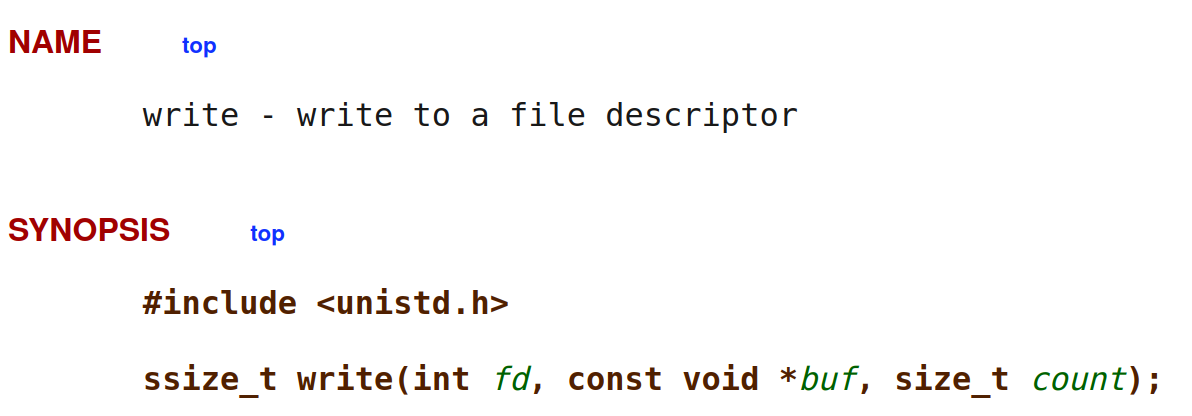
\includegraphics[width=0.8\textwidth]{slides/images/c_api_write.png}
\end{frame}

\begin{frame}[fragile]{OCaml vs C : \texttt{openfile}}
    \begin{lstlisting}
       val openfile : 
            string -> open_flag list -> file_perm -> file_descr
     \end{lstlisting}
    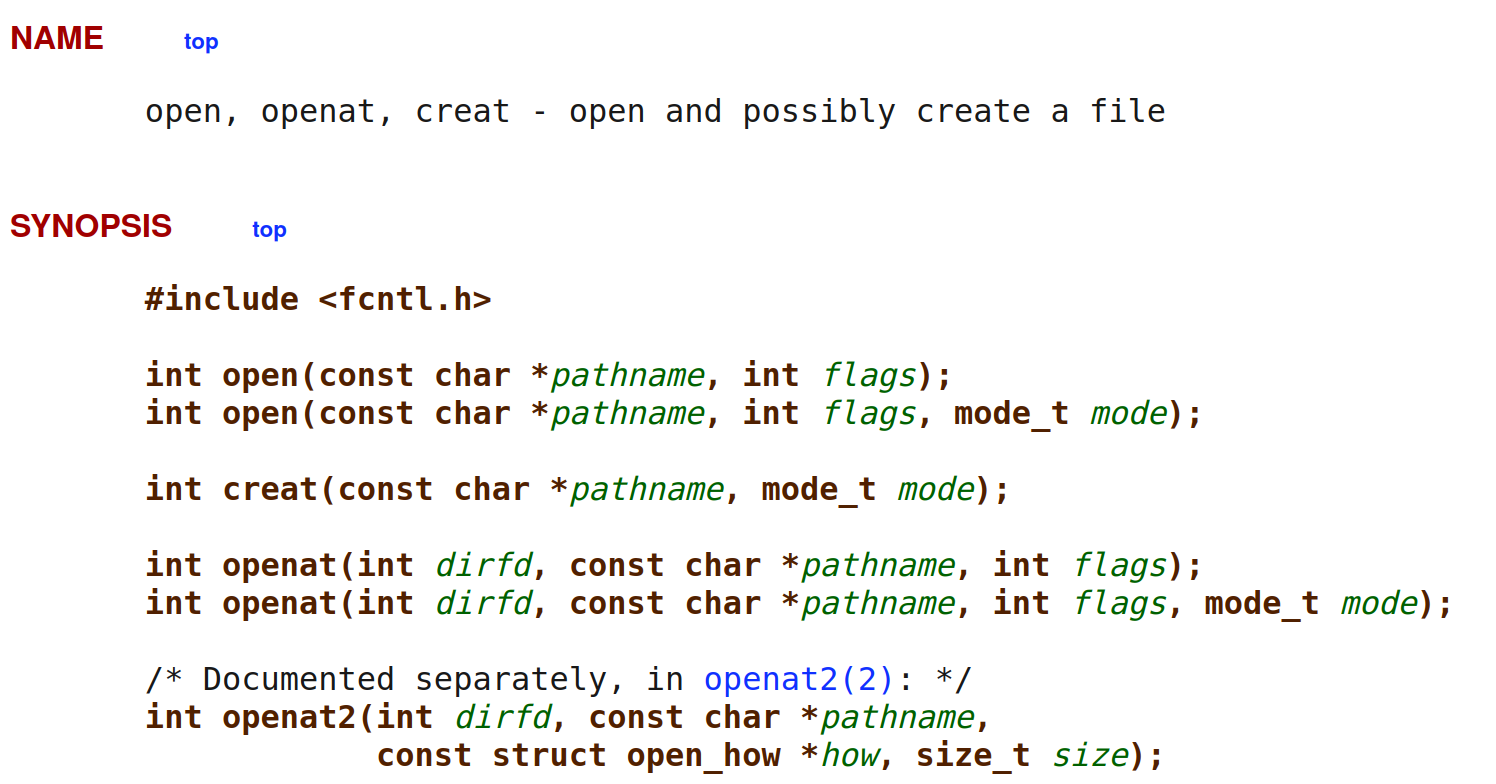
\includegraphics[width=\textwidth]{slides/images/c_api_open.png}
\end{frame}

\begin{frame}[fragile]{Lecture et écriture de fichier (\texttt{cat})}
     \begin{itemize}[label=\small\ding{114}]
         \item pour lire un fichier
             \begin{lstlisting}
                    Unix.openfile filename [O_RDONLY] 0
             \end{lstlisting}
         \item écrire en créant ou en effaçant un fichier existant
             \begin{lstlisting}
                Unix.openfile filename 
                    [O_WRONLY; O_TRUNC; O_CREAT] 0o666
            \end{lstlisting}
        \item écrire du code exécutable
             \begin{lstlisting}
                Unix.openfile filename 
                    [O_WRONLY; O_TRUNC; O_CREAT] 0o777
            \end{lstlisting}
        \item ajouter des données à la fin d'un fichier existant ou le créer vide sinon
             \begin{lstlisting}
                Unix.openfile filename 
                    [O_WRONLY; O_APPEND; O_CREAT] 0o666
            \end{lstlisting}
     \end{itemize} 
\end{frame}

\begin{frame}[fragile]{Lecture et écriture de fichier (\texttt{cat})}
    \begin{itemize}[leftmargin=-10pt]
        \item<2->
            \begin{lstlisting}[basicstyle=\footnotesize\ttfamily]
                let exec_cmd cmd = match cmd with 
                  | Cat files -> 
                    List.iter (fun file ->
                      let fd_in = (* file_perm inutile ici *)
                        Unix.(openfile file [ O_RDONLY ] 0) in
                      write_fd_out fd_in;
                      Unix.close fd_in) files
                  | ... -> ...   
        \end{lstlisting}
        \item<3->
            \begin{lstlisting}[basicstyle=\footnotesize\ttfamily]
                let write_fd_stdout fd_in =
                  let buffer_size = 8192 in
                  let buffer = Bytes.create buffer_size in
                  let rec loop () =
                    match Unix.read fd_in buffer 0 buffer_size with
                    | 0 -> ()
                    | r -> ignore (Unix.(single_write stdout buffer 0 r));
                           loop () in
                  loop ()
            \end{lstlisting}
     \end{itemize}
\end{frame}
\begin{frame}{Opérations sur les noms de fichiers (\texttt{ln (-s)}, \texttt{rm}, \texttt{mv})}
    \texttt{ln f (-s)} : création d'un lien physique (symbolique).

    \texttt{rm f -f} : efface le fichier de nom f

    \texttt{mv f1 f2} : renomme le fichier de nom f1 en f2
    \pause

    \subtt{Exemple}

    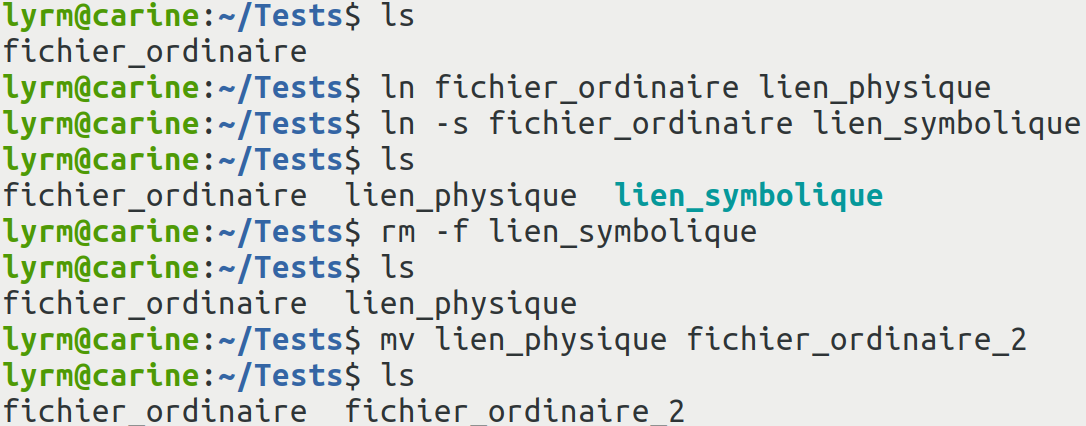
\includegraphics[width=0.7\textwidth]{slides/images/shell_ln_rm_mv.png}
    \pause

    Facile : ce sont des fonctions \texttt{Unix} existantes.
\end{frame}

\begin{frame}[fragile]{Opérations sur les noms de fichiers (\texttt{ln (-s)}, \texttt{rm}, \texttt{mv})}
    \begin{lstlisting}
        (* Efface un fichier *)
        val unlink : string -> unit

        (* Renomme un fichier *)
        val rename : string -> string -> unit

        (* Creer un lien physique *)
        val link : ?follow:bool -> string -> string -> unit

        (* Creer un lien symbolique *)
        val symlink : string -> string -> unit

        (* Lit le contenu d'un lien symbolique *)
        val readlink : string -> string
    \end{lstlisting}
\end{frame}

\begin{frame}[fragile]{Opérations sur les noms de fichiers (\texttt{ln (-s)}, \texttt{rm}, \texttt{mv})}
    \begin{lstlisting}
        let exec_cmd cmd = match cmd with
          | Cat files -> ...

          | Ln (source, dest, symbolic) ->
            if symbolic then Unix.symlink source dest
            else Unix.link source dest

          | Mv (source, dest) -> Unix.rename source dest

          | Rm (filename, recursive) ->
            if recursive then failwith "todo"
            else Unix.unlink filename

          | ... -> ...
    \end{lstlisting}
\end{frame}

\begin{frame}{Opérations sur les répertoires (\texttt{mkdir (-m int)}, \texttt{rm -r}, \texttt{ls})}
     \texttt{mkdir dir (-m int)} : créer un répertoire avec les permissions définies par l'option \texttt{-m}.

     \texttt{rm -r dir} : efface le répertoire nommé \texttt{dir} et son contenu .

    \texttt{ls dir} : liste le contenu du répertoire \texttt{dir} ou du répertoire courant par défault sur la sortie standard.
    \pause

    \subtt{Exemple}

    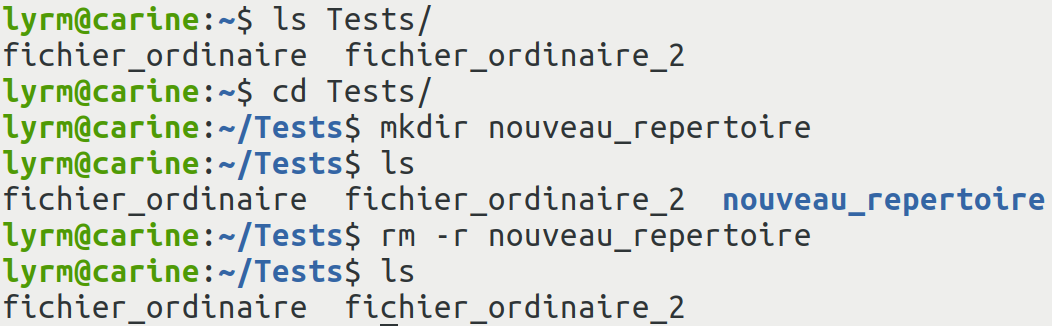
\includegraphics[width=0.8\textwidth]{slides/images/shell_mkdir_rm_ls.png}

\end{frame}

\begin{frame}[fragile]{Opérations sur les répertoires : \texttt{mkdir (-m int)}, \texttt{rm -r}}
    \subtt{Fonctions Unix :}
     \begin{lstlisting}
          type file_perm = int (* ex : 0o777 *)
          val mkdir : string -> file_perm -> unit
          val rmdir : string -> unit
     \end{lstlisting}
    \pause
    \subtt{Implémentation :}
    \begin{lstlisting}
        let exec_cmd cmd = match cmd with
          | Rm (filename, recursive) ->
            if recursive then Unix.rmdir filename
            else Unix.unlink filename
          | Mkdir (filename, perm_opt) -> (* Note : Le parseur ajoute "0o" devant la perm (666 ici) ([mkdir name -m 666])  *)
            let perm = match perm_opt with None -> 0o775 | Some p -> p in
            Unix.mkdir filename perm
          |  ... -> ...
    \end{lstlisting}
\end{frame}

\begin{frame}[fragile]{Opérations sur les répertoires : \texttt{ls}}
    \subtt{Fonctions Unix :}
    \begin{lstlisting}[basicstyle=\scriptsize\ttfamily]
          type dir_handle             (* descripteur de lecture *)
          val opendir : string ->  dir_handle
          val readdir : dir_handle -> string  (* lit une entree *)
          val closedir : dir_handle -> unit
    \end{lstlisting}

    \subtt{Boucle de lecture des entrées du répertoire}
    \begin{lstlisting}[basicstyle=\scriptsize\ttfamily]
    let read_dir dirname =
      let rec loop dir_handle acc =
        try
          let nfile = Unix.readdir dir_handle in
            loop dir_handle (nfile :: acc)
        with End_of_file -> acc in

      let dir_handle = Unix.opendir dirname in (* Ouverture *)
      let files = loop dir_handle [] in          (* Lecture *)
      Unix.closedir direname;                  (* Fermeture *)
      files
    \end{lstlisting}
\end{frame}

\begin{frame}[fragile]{Opérations sur les répertoires : \texttt{ls}}
        \begin{lstlisting}
    let exec_cmd cmd = match cmd with
        | Ls diropt ->
          let dirname = match diropt with
            | None -> Filename.current_dir_name
            | Some d -> d  in
          (* Lecture *)
          let files = read_dir dirname in
          (* Filtrage *)
          let files =  List.filter
              (fun file ->
                not (file = Filename.parent_dir_name ||
                     file = Filename.current_dir_name))
              all_files in
          (* Concatenation *)
          let files = String.concat "\t" files in
          (* Ecriture sur la sortie standard *)
          write_stdout (files ^ "\n")
        | ... -> ...
        \end{lstlisting}
\end{frame}

\begin{frame}[fragile]{Opérations sur les répertoires : \texttt{ls}}

    La fonction d'écriture sur la sortie standard ressemble beaucoup à celle vue précédemment :
    \begin{lstlisting}
        let write_stdout text =
          (* Conversion en bytes *)
          let text = Bytes.of_string text in
          (* Taille max du bloc d'ecriture *)
          let max_len = 8192 in
          (* boucle d'ecriture *)
          let rec loop ind to_write =
            let len = min max_len to_write in
            let written = Unix.single_write Unix.stdout text ind len in
            if written = max_len then
              loop (ind + written) (to_write - written)
          in
          loop 0 (Bytes.length text)
    \end{lstlisting}
\end{frame}

\begin{frame}[fragile]{Opérations sur les répertoires : \texttt{ls}}
    \subtt{Ajouter l'option \texttt{-i} pour \texttt{ls}}

    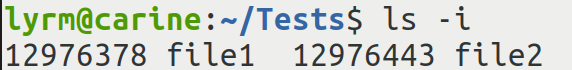
\includegraphics[width=0.5\textwidth]{slides/images/shell_ls_inode.png}

    \begin{lstlisting}
      type stats = {
	st_dev : int; (* Numéro de périphérique *)
	st_ino : int; (* Numéro d'Inode *)
	st_kind : file_kind; (* Type de fichiers (S_REG, S_DIR) *)
	st_perm : file_perm; (* Droits *)
	... }

      (* Information sur le fichier *)
      val stat : string -> stats
      (* Comme [stat] avec un descripteur de fichier *)
      val fstat : file_descr -> stats
      (* Donne l'information sur un lien symbolique *)
      val lstat : string -> stats
    \end{lstlisting}

\end{frame}

\subsection{Gestion des erreurs Unix et boucle principale de lecture}

\begin{frame}[fragile]{Gestion des erreurs}
  \subtt{En C}, pour chaque appel système :
  \begin{lstlisting}[language=C]
    if (unappel() == -1) {
      printf("unappel() a échoué\n");
      if (errno == ...) { ... }}
  \end{lstlisting}
  \pause
  \subtt{Avec OCaml,} une fois à la fin du programme
  \begin{lstlisting}
    type error = | E2BIG | EACCES | EAGAIN | EBADF | ...
    val handle_unix_error : ('a -> 'b) -> 'a -> 'b
  \end{lstlisting}
  \pause
  \footnotesize
  \begin{itemize}[label=\small\ding{114}]
       \item applique le premier argument (notre programme) au second
         et retourne le résultat.
       \item Si une exception \texttt{Unix.Unix\_error} est levée :
         \begin{itemize}[label=\ding{118}]
         \item affiche une message décrivant l'erreur
         \item le programme termine avec le code d'erreur 2
         \end{itemize}
    \end{itemize}
\end{frame}

\begin{frame}[fragile]{Boucle principale de lecture : premier essai}
  \begin{itemize}
    \item<1->
    \begin{lstlisting}
      let minishell () =
    \end{lstlisting}
    \item<2-> \begin{itemize} \item \begin{lstlisting}
      try
        while true do
          let cmd_line = Stdlib.input_line Stdlib.stdin in
          try
            let cmd = parse cmd_line in
            exec_cmd cmd
          with
          | Parsing_error err -> print_error err
          | Empty_line -> ()
        done
      with End_of_file -> ()
    \end{lstlisting} \end{itemize}
    \item <1->
    \begin{lstlisting}
      let () = Unix.handle_unix_error minishell ()
    \end{lstlisting}
    \end{itemize}
\end{frame}

\subsection{Redirection et tube}
\begin{frame}{Processus}

\begin{columns}
  \column{0.38\linewidth}
\begin{figure}
    \centering
    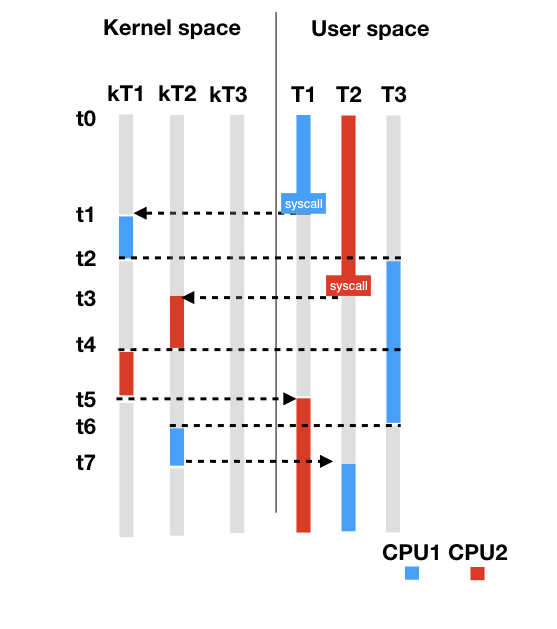
\includegraphics[width=\textwidth]{slides/images/scheduling.jpg}
\end{figure}

\column{0.58\linewidth}

\subtt{État d'un processus}

 \begin{itemize}[label=$-$]
     \item Registres processeur
     \item Table des descripteurs fichiers
     \item Répertoire courant
     \item Variables d'environnement
 \end{itemize}
\end{columns}

\end{frame}

\begin{frame}{\texttt{fork}}

    fonction Unix.fork : unit -> int

    crée un nouveau process avec le même état
\end{frame}

\begin{frame}[fragile]{Boucle de lecture avec gestion des erreurs}
\begin{lstlisting}
    let minishell () =
        try
           while true do
             (* Lecture de l'entree standard *)
             let cmd = input_line Stdin.stdin in
             match Unix.fork () with
               | 0 ->
                 (* Processus fils *)
                 let cmd = parse cmd_line in
                 exec_cmd cmd;
                 exit 0
               | pid_son ->
                 (* Processus pere *)
                 let pid, status = Unix.wait() in
                 (* Affiche le status de sortie du processus père *)
                 print_status "Program" status
          done
          with End_of_file -> ()

    let () = Unix.handle_unix_error minishell ()
\end{lstlisting}
\end{frame}

\begin{frame}[fragile]{AST évolué}
    \begin{itemize}[leftmargin=-10pt]
         \item
        \begin{lstlisting}
            type cmd_kind =
                | Internal of command (* les commandes precedentes *)
                | External of string list (* la triche avec execv *)
                | Cd of string (* getcwd / chdir *)
            type redirection =
                | In of string (* > *)
                | Out of string (* < *)
            type command = cmd_kind * redirection list
            type t =
                | Command of command
                | Pipe of t * t (* | *)
                | And of t * t (* exit status *)
                | Or of t * t
            val execute : t -> unit
        \end{lstlisting}
    \end{itemize}

\end{frame}


\begin{frame}[fragile]{AST évolué}
    \begin{itemize}[leftmargin=-10pt]
         \item
        \begin{lstlisting}
            type cmd_kind =
                | Internal of command (* les commandes precedentes *)
                | External of string list (* la triche avec execv *)
                | Cd of string (* getcwd / chdir *)
            type redirection =
                | In of string (* > *)
                | Out of string (* < *)
            type command = cmd_kind * redirection list
            type t =
                | Command of command
                | Pipe of t * t (* | *)
                | And of t * t (* exit status *)
                | Or of t * t
            val execute : t -> unit
        \end{lstlisting}
    \end{itemize}

\end{frame}

\begin{frame}[fragile]{Nouvelle boucle de lecture}
\begin{lstlisting}
let minishell () =
 try
     Printf.printf "%s> %!" (Unix.getcwd ());
     while true do
       let cmd = input_line Stdlib.stdin in
       try
         let cmd = Ast.parse cmd in
         let code = interprete cmd in
         Printf.printf "%s (%d)> %!" (Unix.getcwd ()) code
       with
       | Parser.Parsing_error err -> Parser.print_error err
       | Parser.Empty_line -> ()
     done
   with End_of_file -> ()
\end{lstlisting}
\end{frame}

\begin{frame}{}

\end{frame}

\begin{frame}{\texttt{cd}}

\end{frame}

\begin{frame}{\texttt{fork}}

\end{frame}


\subsection{Manipulation de fichiers et répertoires}
\begin{frame}[fragile]{Redirections}

\begin{columns}

\column{0.38\linewidth}
\begin{figure}
    \centering
    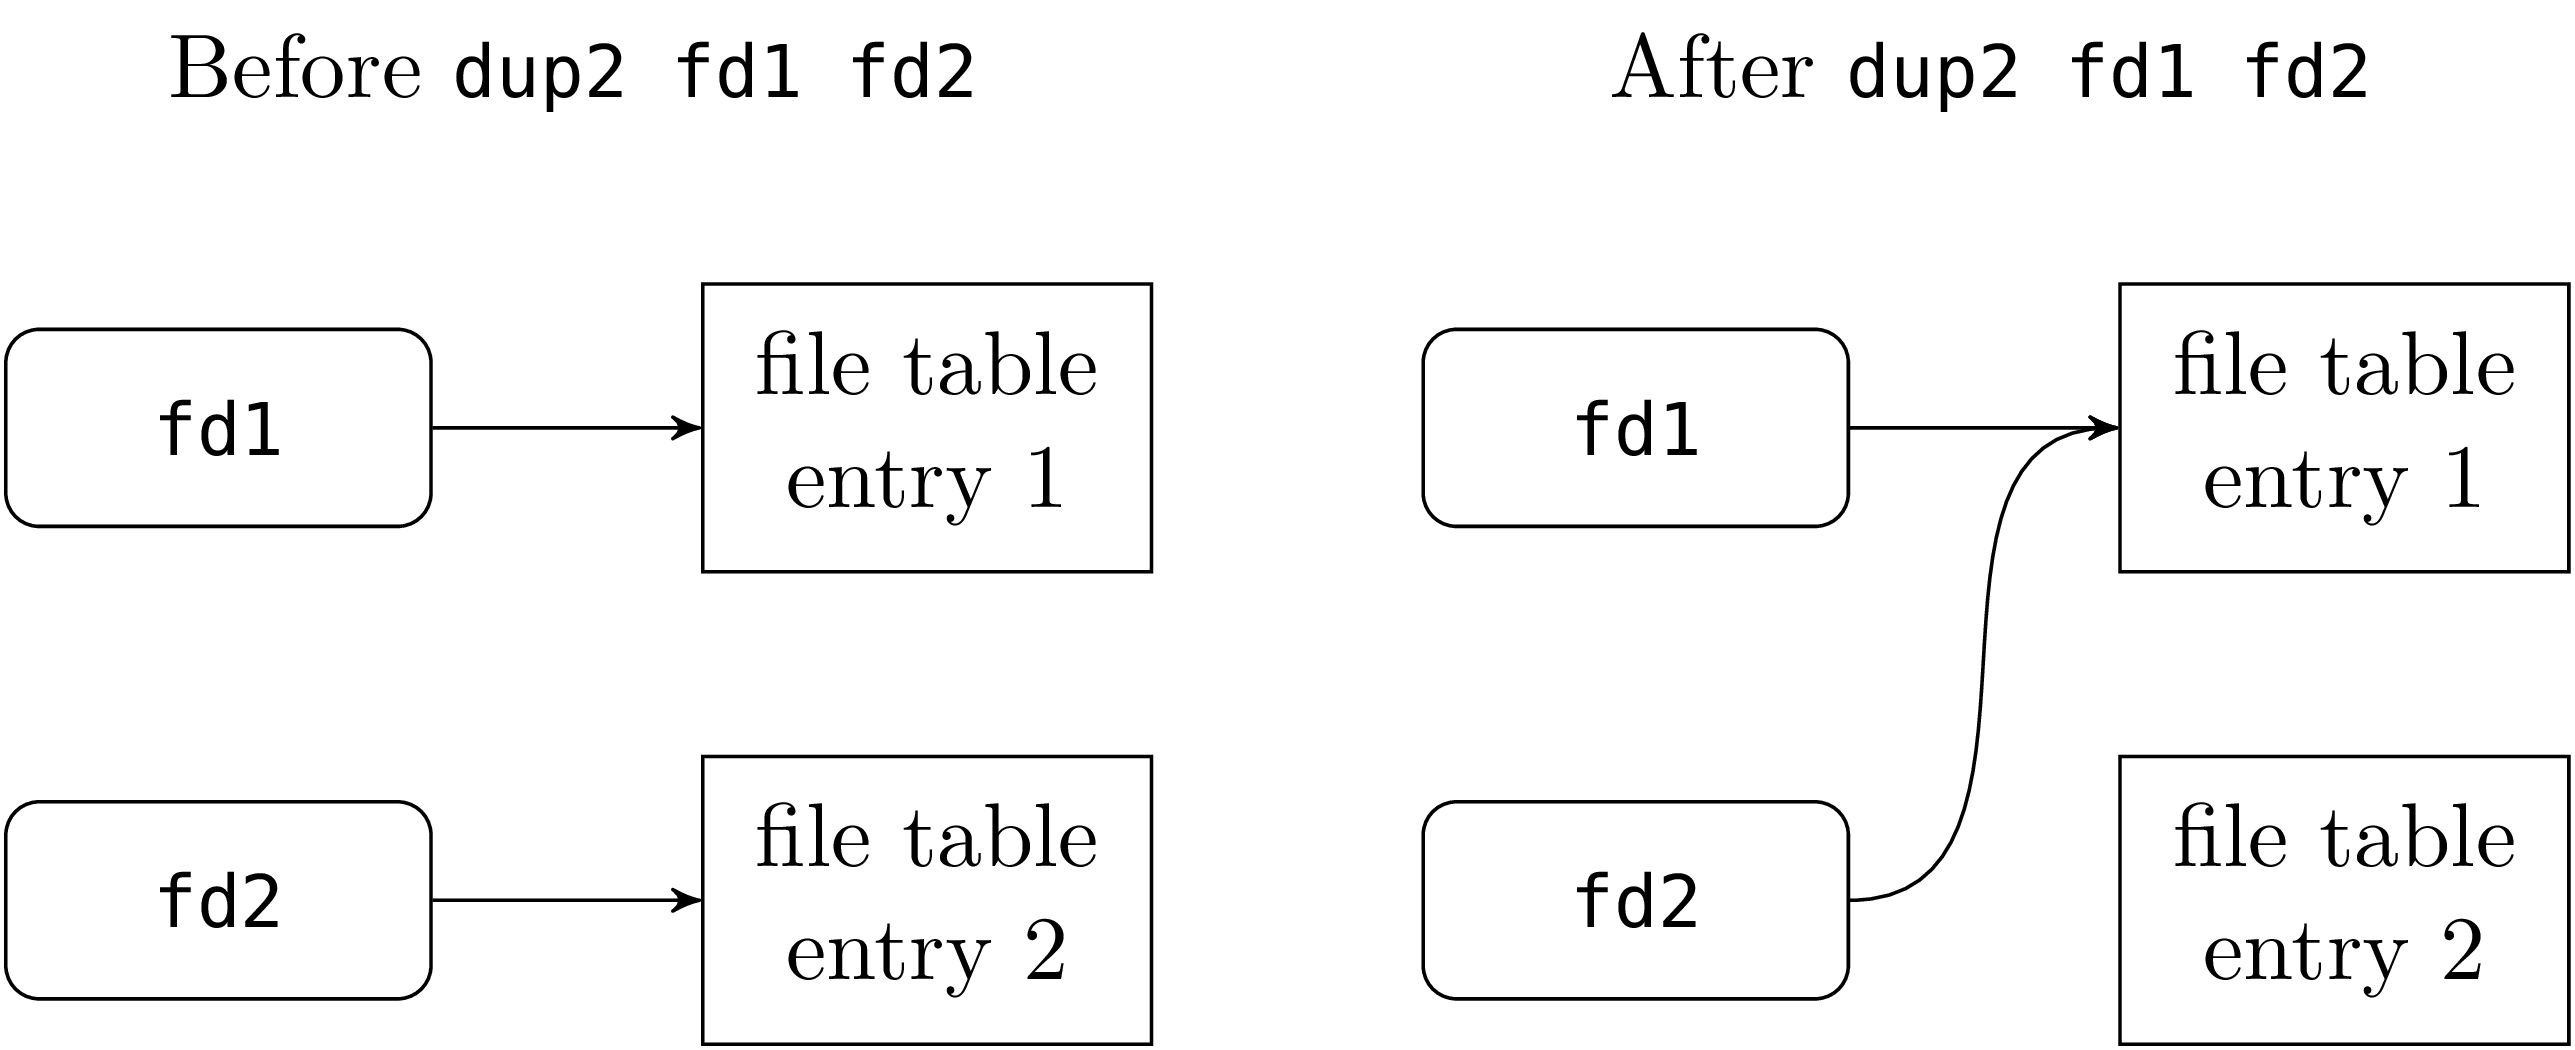
\includegraphics[width=\textwidth]{slides/images/dup2.png}
\end{figure}

\column{0.58\linewidth}
\\
\subtt{Fonction Unix:}
\begin{lstlisting}
val dup2 : file_descr -> file_descr -> unit
\end{lstlisting}

\end{columns}

\subtt{Implémentation :}

\begin{lstlisting}
let redirection_entree target =
  let fd = Unix.openfile target [ Unix.O_RDONLY ] 0 in
  Unix.dup2 fd Unix.stdin;
  Unix.close fd

let redirection_sortie target =
  let fd = Unix.openfile target [ Unix.O_CREAT ; 
                                  Unix.O_TRUNC ; 
                                  Unix.O_WRONLY ] 0o660
  in
  Unix.dup2 fd Unix.stdout;
  Unix.close fd
\end{lstlisting}

\end{frame}

\begin{frame}[fragile]{Tubes}

\subtt{Fonction Unix :}
\begin{lstlisting}
val pipe : unit -> file_descr * file_descr
\end{lstlisting}

\subtt{Implémentation :}
\begin{lstlisting}
let pipe_cmd (a: Command.t) (b: Command.t) =
  let fd_in, fd_out = Unix.pipe () in
  match Unix.fork () with
  | 0 ->
      Unix.dup2 fd_out Unix.stdout;
      Unix.close fd_out;
      Unix.close fd_in;
      interprete a
  | _ ->
      Unix.dup2 fd_in Unix.stdin;
      Unix.close fd_out;
      Unix.close fd_in;
      interprete b
\end{lstlisting}

\end{frame}

\subsection{Interlude réseau}
\input{slides/systeme_6_réseau}

\subsection{Programme système avancée}

\begin{frame}[fragile]{Interactions haut niveau avec le système}
 
\subtt{Le module \texttt{Stdlib} contient des primitives haut niveau pour la manipulation de fichiers}

\begin{lstlisting}
type in_channel
type out_channel

val open_in : string -> in_channel
val input_line : in_channel -> string
val close_in : in_channel -> unit

val open_out : string -> out_channel
val output_string : out_channel -> string -> unit
val close_out : in_channel -> unit

\end{lstlisting}
    
\end{frame}

\begin{frame}{Programmation asynchrone}
Le problème des appels en système de lecture/écriture : c'est bloquant.
 
Plusieurs stratégies:
\begin{itemize}[label=\small\ding{114}]
    \item Utiliser des fils d'exécution (threads)
    \item \texttt{Lwt}: bibliothèque pour fils d'exécutions légers et coopératifs
\end{itemize}
\end{frame}

\begin{frame}[fragile]{Exemple: \texttt{cp} asynchrone avec \texttt{Lwt\_unix}}

\begin{lstlisting}
open Lwt.Syntax

let rec perform_copy_lwt src dst =
  let* n = Lwt_unix.read src buffer 0 buf_size in
  if n = buf_size then
    let* _ = Lwt_unix.write dst buffer 0 n in
    perform_copy_lwt src dst
  else
    let* _ = Lwt_unix.write dst buffer 0 n in
    Lwt.return (`Ok ())

let cp_lwt src dest =
  Lwt_main.run @@
  let* fd_src = Lwt_unix.openfile src [O_RDONLY] 0 in 
  let* fd_dst = Lwt_unix.openfile dest [O_RDWR; O_CREAT; O_TRUNC] 0o640 in
  perform_copy_lwt fd_src fd_dst
\end{lstlisting}
    
\end{frame}

\section{OCaml dans la vraie vie}

\begin{frame}{OCaml IRL}

\begin{enumerate}[label=\small\ding{114}]
    \item MirageOS: un système d'exploitation modulaire écrit en OCaml
    \item OCaml 5: programmation parallèle (et effets)
    \item QCheck: vérification de propriétés automatique
    \item Écosystème et environnements de programmation
\end{enumerate}
    
\end{frame}

\subsection{Mirage}

\begin{frame}{MirageOS}
    
\begin{figure}
    \centering
    \begin{minipage}{0.45\textwidth}
        \centering
        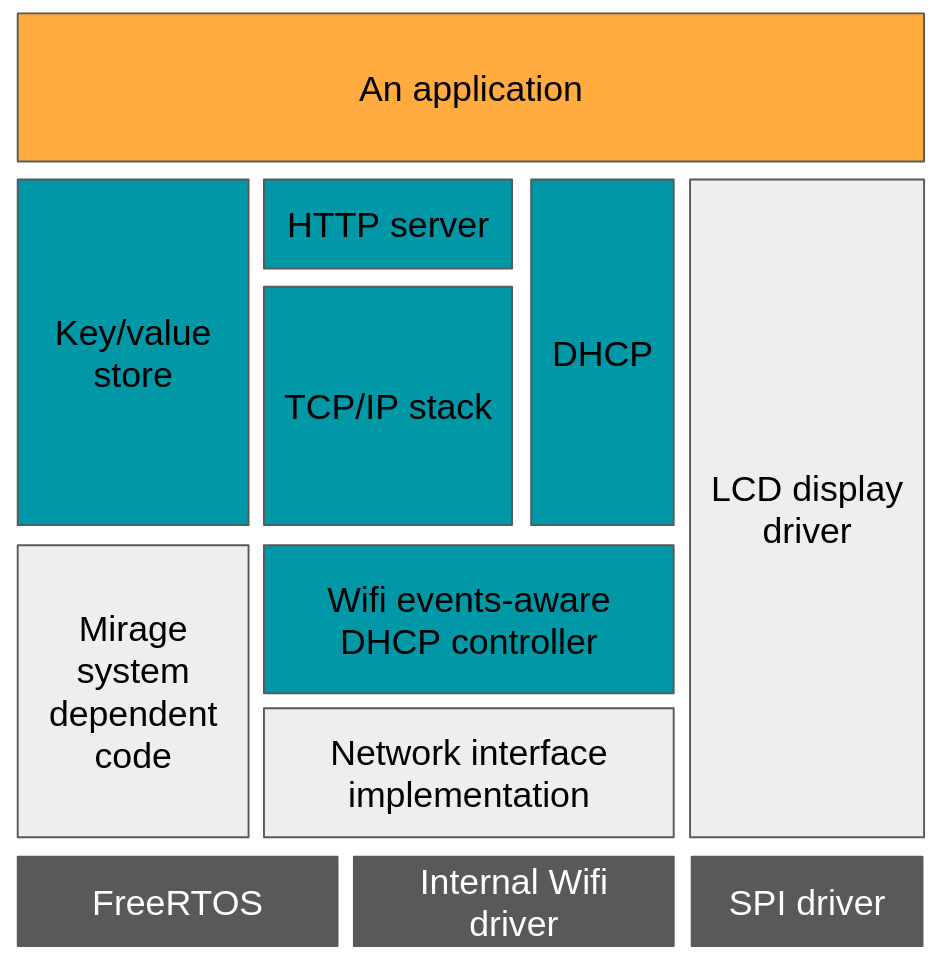
\includegraphics[width=0.9\textwidth]{slides/images/mirage.png}
        \caption{Une application modulaire}
    \end{minipage}\hfill
    \begin{minipage}{0.45\textwidth}
        \centering
        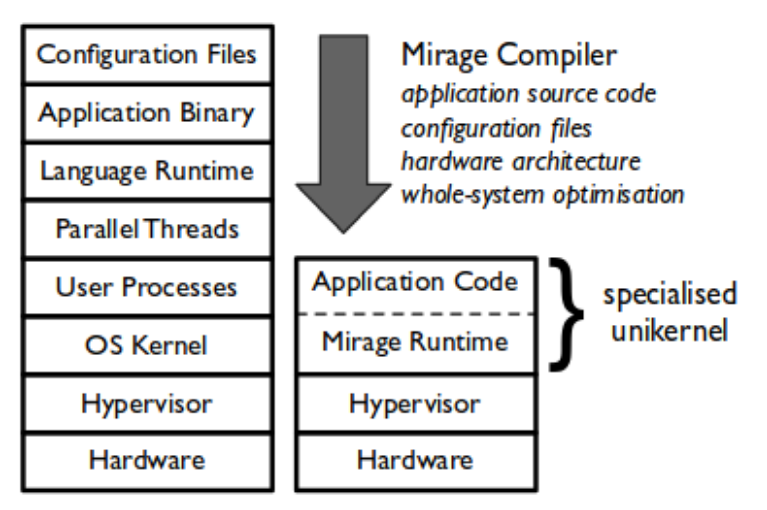
\includegraphics[width=0.9\textwidth]{slides/images/mirage2.png}
        \caption{MirageOS compile à la fois l'application et le système dans un seul exécutable}
    \end{minipage}
\end{figure}

\end{frame}

\begin{frame}[fragile]{Abstraction: signatures de modules}

\begin{lstlisting}
module type Read_only_store = sig 
    type t
    type key = string
    
    val get : t -> key -> string Lwt.t
end
\end{lstlisting}

\begin{lstlisting}
module type HTTP = sig
    type t
    module Request : sig 
        type t
        
        val path : t -> string
    end
    type reponse = string
    
    val listen : t -> (HTTP.Request.t -> response Lwt.t) -> unit Lwt.t
end
\end{lstlisting}


\end{frame}

\begin{frame}[fragile]{Implémentation}
    
\begin{lstlisting}

(* les dependances de notre application sont abstraites 
   via le foncteur Make *)
module Make (FS : Read_only_store) (Server : HTTP) = 
struct
    let start fs http =
        HTTP.listen http (fun request ->
            let path = HTTP.Request.path request in
            FS.get fs path)
end

(* pour les tests *)
module Application = Make (In_memory_store) (Mock_http_server)

(* en production *)
module Application = Make (EXT4) (Cohttp.Server)
\end{lstlisting}

\end{frame}

\begin{frame}{Modules disponibles}
\begin{enumerate}[label=$-$]
    \item Socket réseau: TCP/IP de l'OS ou en OCaml
    \item Stockage: en mémoire, Irmin, FAT
    \item Protocoles: Git, HTTP, SSH, DNS, DHCP
    \item Cryptographie / compression
\end{enumerate}
\end{frame}

%\begin{frame}[fragile]{Boucle d'événements}
%
%\begin{lstlisting}
%val run : unit Lwt.t -> unit
%\end{lstlisting}
%
%\begin{lstlisting}
% let run t =
%   let rec aux () =
%     Time.restart_threads Time.time;
%     match Lwt.poll t with
%     | Some () -> ()
%     | None ->
%         let timeout = Time.select_next () in
%         let ready_set = solo5_yield timeout in
%         (if ready_set <> 0L then
%          (* Some I/O is possible, wake up threads and continue. *)
%          wakeup_threads ready_set);
%         aux ()
%   in
%   aux ()
% \end{lstlisting}
% \end{frame}

\subsection{OCaml Multicore}

\begin{frame}{OCaml 5}


\begin{figure}
    \centering
    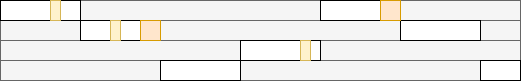
\includegraphics[width=0.9\textwidth]{slides/images/concurrence.png}
    \caption{Concurrence}
\end{figure}

\begin{figure}
    \centering
    \includegraphics[width=0.9\textwidth]{slides/images/parallélisme.png}
    \caption{Parallélisme}
\end{figure}
% Blanc = code OCaml
% Jaune = minor GC
% Orange = major GC
\end{frame}

\begin{frame}{Peterson}
    
\end{frame}

\begin{frame}{Lamport}
    
\end{frame}

\subsection{Vérification de propriétés avec QCheck}

\begin{frame}[fragile]{QCheck}
    
Vérification de propriétés

\begin{figure}
    \centering
    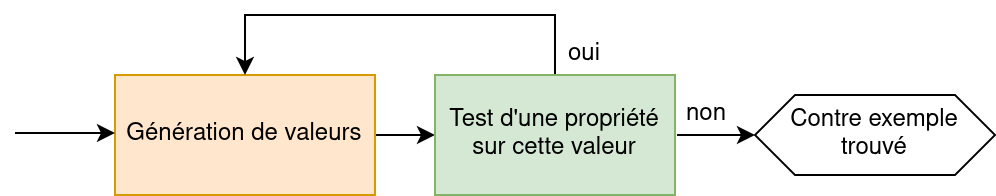
\includegraphics[width=0.9\textwidth]{slides/images/qcheck.drawio.png}
\end{figure}

\subtt{QCheck cherche un contre exemple minimal}

\begin{lstlisting}
type 'a generator
val small_int : int generator
val small_list : 'a generator -> 'a list generator
val Test.make : 'a generator -> ('a -> bool) -> Test.t
\end{lstlisting}

Plus d'informations: \url{https://github.com/c-cube/qcheck}
\end{frame}

\begin{frame}[fragile]{Exemple de test}

\begin{lstlisting}

let generateur = QCheck.(small_list small_int)
\end{lstlisting}

\subtt{Inverser une liste}
\begin{lstlisting}
let predicat entree sortie =
    let entree = Array.of_list entree in
    let sortie = Array.of_list sortie in
    let n = Array.length entree in
    assert (n = Array.length sortie);
    for i = 0 to n - 1 do
      assert (entree.(i) = sortie.(n-1-i))
    done;
    true
\end{lstlisting}

\subtt{Trier une liste}
\begin{lstlisting}
let predicat entree sortie =
    List.sort Int.compare entree = sortie
\end{lstlisting}

\end{frame}

\begin{frame}[fragile]{Réduction}
    
\begin{lstlisting}
  let inverser lst = 
    if List.length lst >= 5 then lst
    else List.rev lst
\end{lstlisting}
\subtt{Réduction du contre exemple}
\begin{lstlisting}
0   => [3176607639030078719; -702777917135807191; 1243225506173352439; -168141035741141589; 4478591693389419378; -2908482084465810011; -4471604993596125836; 2097048314685490782; -777119667999583759]
1   => [1243225506173352439; -168141035741141589; 4478591693389419378; -2908482084465810011; -4471604993596125836; 2097048314685490782; -777119667999583759]
200 => [0; 0; 0; 4095797489620100; -777119667999583759]
255 => [0; 0; 0; 0; -194279916999895940]
299 => [0; 0; 0; 0; -11044]
313 => [0; 0; 0; 0; -1]
\end{lstlisting}

\end{frame}

\begin{frame}{Simulation d'un état}

\begin{figure}
\centering
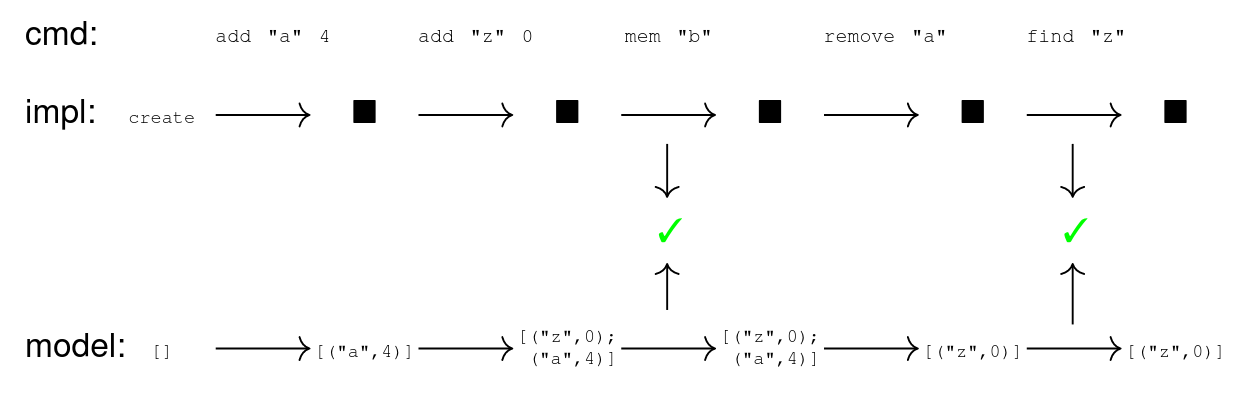
\includegraphics[width=\textwidth]{slides/images/qcheck_state.png}
\end{figure}
\begin{figure}
\centering
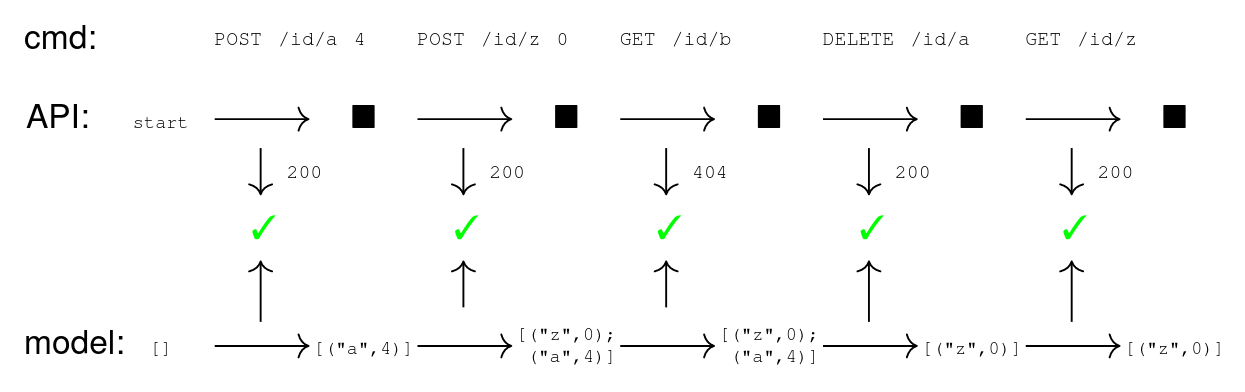
\includegraphics[width=\textwidth]{slides/images/qcheck_state_2.png}
\end{figure}

\end{frame}
\subsection{Écosystème}
\input{slides/irl_4_ecosystème}

\end{document}
